\documentclass{article}
\usepackage{graphicx}
\usepackage{subcaption}
\usepackage[margin=1in]{geometry}
\usepackage{gensymb}

\begin{document}

\begin{figure}[ht]
\centering
\begin{subfigure}{0.3\linewidth}
	\centering
	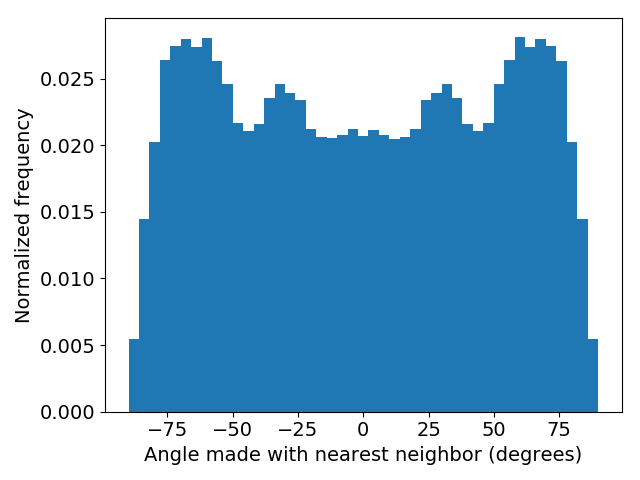
\includegraphics[width=\linewidth]{offset_tail_packing.png}
	\caption{}~\label{fig:offset_tails}	
\end{subfigure}
\begin{subfigure}{0.3\linewidth}
	\centering
	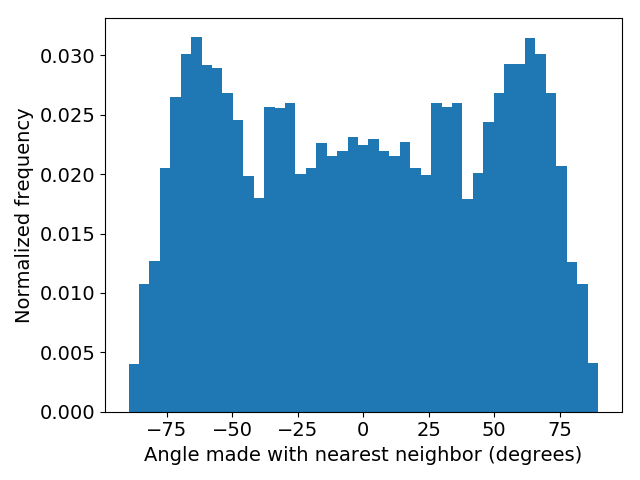
\includegraphics[width=\linewidth]{angles_traj_layered.png}
	\caption{}~\label{fig:layered_tails}
\end{subfigure}
\begin{subfigure}{0.3\linewidth}
	\centering
	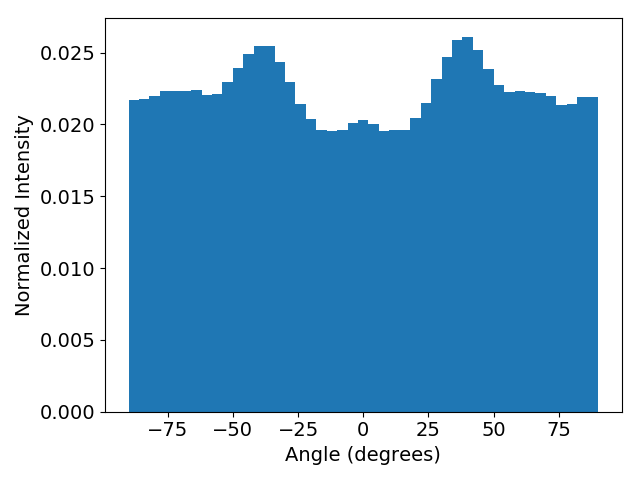
\includegraphics[width=\linewidth]{integrated_WAXS_ring.png}
	\caption{}~\label{fig:rz_layered}
\end{subfigure}
\caption{The distribution of angles w.r.t. xy plane between alkane chain tail centroids and nearest 
neighbor centroids for equilibrated parallel displaced (a) and sandwiched (b) configurations both show 
distinct peaks at $\pm$ 33 $\degree$. (c) Integrated 2D WAXS data between $q_r$=1 and $q_r$=1.42 shows
distinct peaks at with maxima at $\pm$ 37 $\degree$}~\label{fig:tail_packing}
\end{figure}

\end{document}
